\documentclass[12pt]{article}
\usepackage[utf8]{inputenc}
\usepackage{amsmath}
\usepackage[T1]{fontenc}

\title{ECE 3413 Lab 09\\*DC Motor Model for PID Feedback Control in MATLAB Simulink}
\author{Leomar Dur\'an}
\date{${19}^{\text{th}}$ April 2023}

\usepackage[natbib,style=apa6]{biblatex}
\addbibresource{main.bib}
\defbibheading{bibliography}[\refname]{%
  \section*{\centering #1}%
}%

\usepackage{hyperref}

\usepackage{cancel}
\usepackage[per-mode=symbol]{siunitx}
\newcommand*\siexpr[2][]{\SI[parse-numbers=false,#1]{#2}}%
\usepackage{xfrac}
\usepackage{amssymb}
\newcommand*\transpose{\mathsf{T}}

\usepackage{mathtools}%
\DeclarePairedDelimiter\brao()%
\DeclarePairedDelimiter\brac[]%
\DeclarePairedDelimiter\braco[)%
\DeclarePairedDelimiter\braoo][%
\DeclarePairedDelimiter\Brac\{\}%
\DeclarePairedDelimiter\abs||
\DeclarePairedDelimiter\norm\lVert\rVert%
\DeclarePairedDelimiter\piecefn\{.
\DeclarePairedDelimiter\evalat.|

\usepackage{lib/nonfloatenvirons}
\usepackage{booktabs}
\newcommand\ra[1]{\renewcommand*\arraystretch{#1}}
\ra{1.25}

\usepackage{minted}
\newcommand\matlab{matlab}

\usepackage{adjustbox}
\newcommand{\setprime}[2][1]{%
    {#2}^{%
        \raisebox{1pt}{%
            \scalebox{0.5}{%
                \itshape\sffamily\uppercase%
                \expandafter{%
                    \romannumeral#1%
                }%
            }%
        }
    }%
}%
\newcommand*\mcadj[7]%
% {#columns}{col spec}{rotation}{adjust spec}
% {before rotated text}{rotated text}{after rotated text}
{%
    \multicolumn{#1}{#2}{%
        \rlap{%
            #5\adjustbox{rotate=#3,#4}{#6}~#7%
        }%
    }%
}

\usepackage{pdfpages}
\usepackage{standalone}
\usepackage{matlab}

\usepackage[skip=\baselineskip,indent=0pt]{parskip}
\setlength\parindent{0pt}

\usepackage[shortlabels]{enumitem}

\def\hr{{\par\noindent\rule{\textwidth}{0.4pt}}}

\begin{document}

\maketitle
\newpage

\section{Introduction}

This experiment builds on the previous lab (DC Motor Model for Open-loop Control in MATLAB Simulink) by providing a PID (proportional-integral-derivative) feedback controller to stabilize the angular velocity.

As we saw earlier, the angular velocity will rise increasingly until it reaches the desired velocity and plateaus. Fig.~\ref{fig:plot of angular velocity} shows this increment of angular velocity.

\begin{figure}
    \centering
    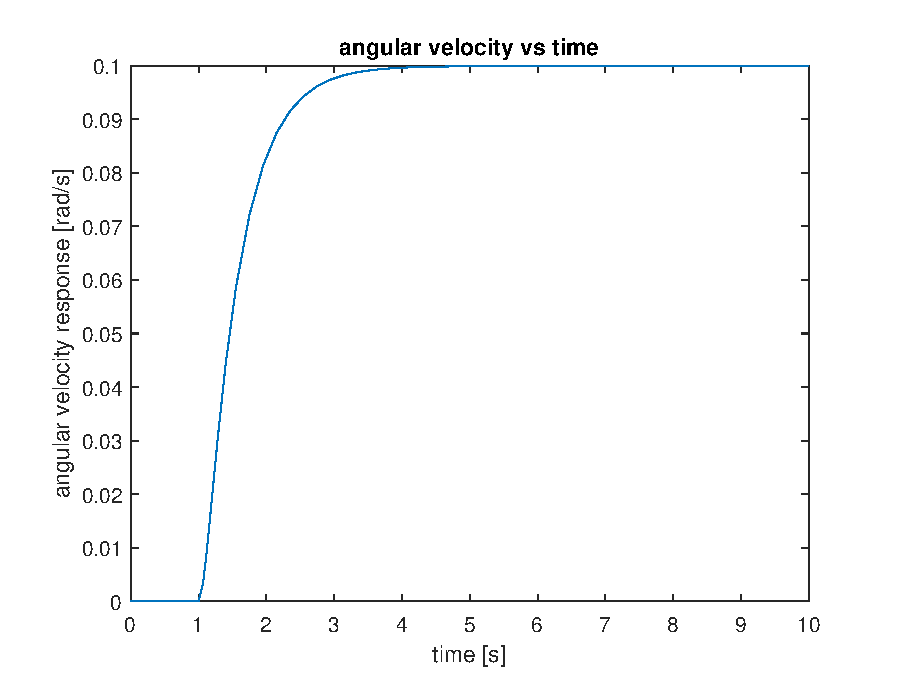
\includegraphics[width=\linewidth]{img/task02_plot_angular_velocity.eps}
    \caption{Plot of the angular velocity response.}
    \label{fig:plot of angular velocity}
\end{figure}

From this, we can expect the angular position to increase equally throughout the runtime as we see in Fig.~\ref{fig:angular position of motor}.

\begin{figure}
    \centering
    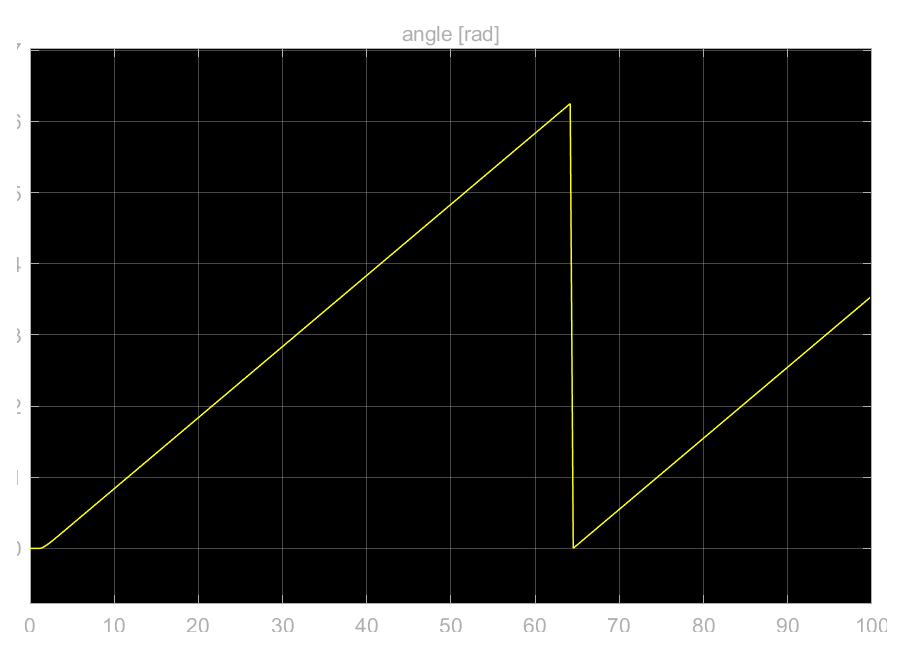
\includegraphics[width=\linewidth]{img/task05_angular_position.eps}
    \caption{The angular position of the motor.}
    \label{fig:angular position of motor}
\end{figure}

However, it may be desired to change the output of the motor. In which case, we can use a PID controller to stabilize this change according to whichever parameter we desire.

These parameters may include wanting the system to be overdamped (for more stead changes) or underdamped (for quicker changes).

\section{Procedure}\label{sec:procedure}

\subsection{Task 0 -- Adding the PID controller}\label{ssc:dc motor model}

We start with the DC motor model from the previous lab as shown on pages~\pageref{pdf:dc motor model} and \pageref{pdf:integrators}.

However, to the original system from lab~08, we are adding a PID controller and a negative unit feedback loop as seen on page~\ref{pdf:PID controller system}.

\begin{figure}
    \centering
    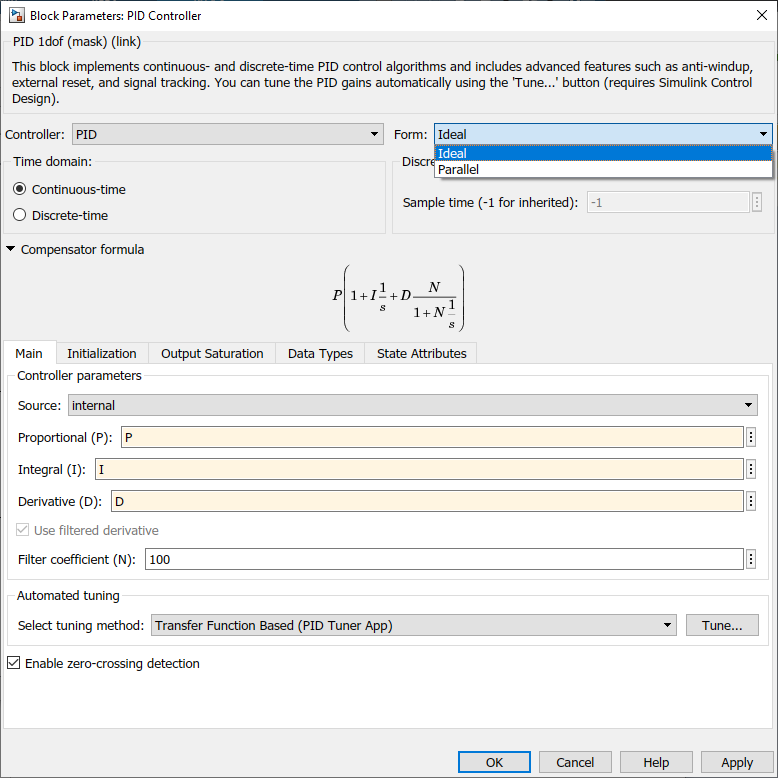
\includegraphics[width=\linewidth]{img/task00_010_setting_up_PID_controller.png}
    \caption{Setting up the PID controller.}
    \label{fig:pid controller block parameters}
\end{figure}

Additionally, to set up the PID controller, we must edit the block parameters as seen in Fig.~\ref{fig:pid controller block parameters}. We have made the following changes:
\begin{enumerate}
    \item Change the Form from ``Parallel'' to ``Ideal''.
    \item Set Proportional (P) to \mintinline\matlab{P}.
    \item Set Integral (I) to \mintinline\matlab{I}.
    \item Set Derivative (D) to \mintinline\matlab{D}.
\end{enumerate}

We can see the general form of the compensator formula here, that is
\begin{equation}
    P\brao*{1 + I\frac1s + D\frac{N}{\displaystyle1 + N\frac1s}}.
\end{equation}

\begin{figure}
    \centering
    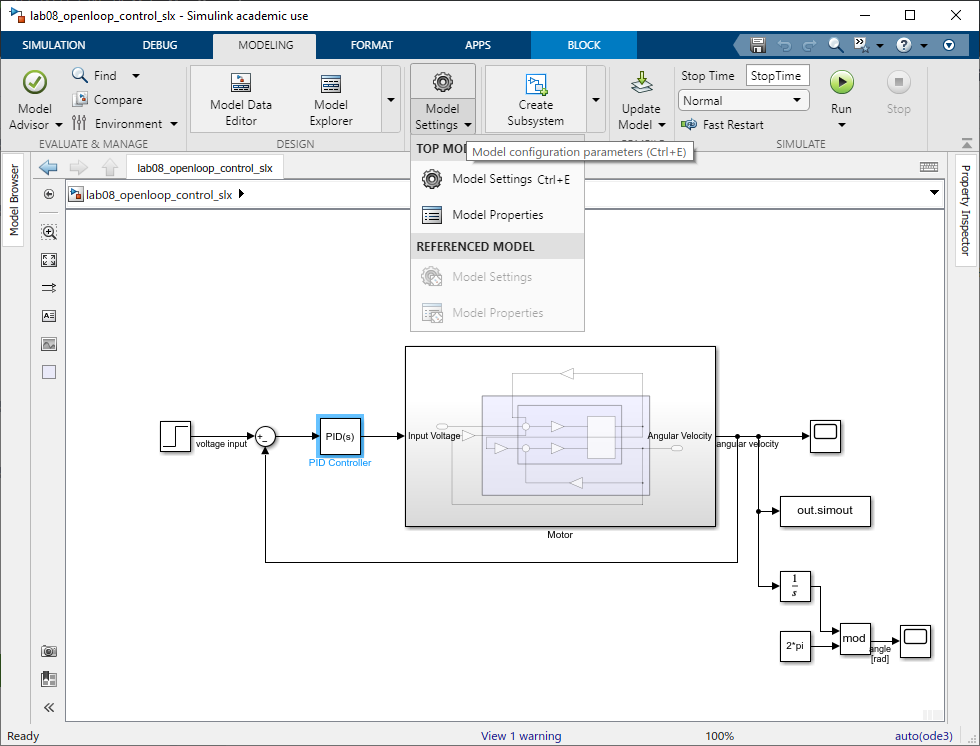
\includegraphics[width=\linewidth]{img/task00_020_finding_model_settings.png}
    \caption{Locating the model settings.}
    \label{fig:task00_020_finding_model_settings}
\end{figure}

\includepdf[pages=2,landscape=true,pagecommand=\label{pdf:dc motor model}]{drawings/lab09_pid_feedback_control_slx.pdf}
\includepdf[pages=3,landscape=true,pagecommand=\label{pdf:integrators}]{drawings/lab09_pid_feedback_control_slx.pdf}
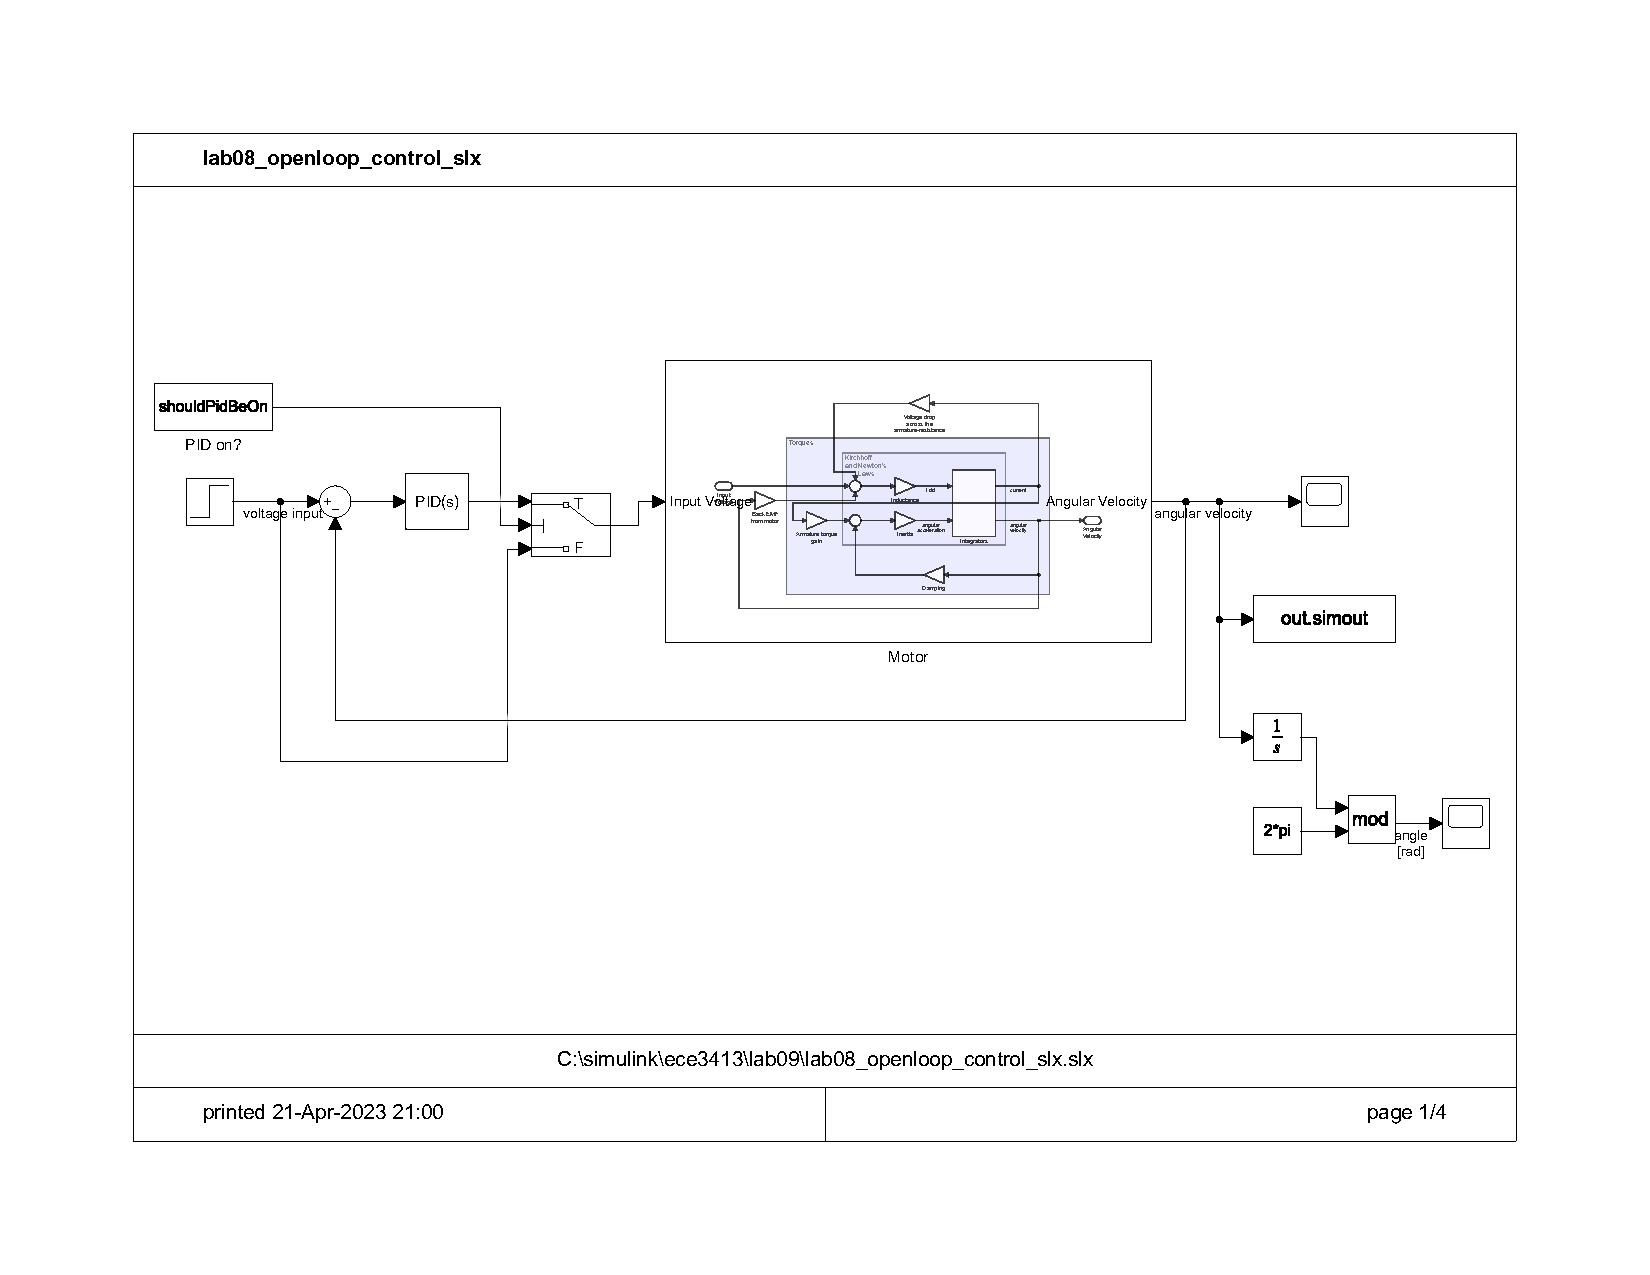
\includepdf[pages=1,landscape=true,pagecommand=\label{pdf:PID controller system}]{drawings/lab09_pid_feedback_control_slx.pdf}

We will also need to change the Model Settings. These can be found by clicking on the ``MODELING'' tab at the top of the Simulink window. Then selecting the Model Settings with the gear icon near the middle as see in \ref{fig:task00_020_finding_model_settings}.

The settings that we changed are as follows:
\begin{enumerate}
    \item Add a Start time of \mintinline\matlab{StartTime}.
    \item Set the Solver selection to ``Fixed-step''.
    \item Set the Fixed-step size, which is the sampling frequency to \mintinline\matlab{Fs}.
\end{enumerate}

Now these settings are all parameterized by the script in \nameref{app} Subsection~\ref{sap:initial params}.

\subsection{Task 1 -- Varying the proportional terms}

We plotted the result of modeling the PID feedback system as a purely proportional system with the proportional terms given in \eqref{eq:proportional}.

\begin{equation}\label{eq:proportional}
    P \in \Brac*{10^n\middle| n \in 0..3^{\vphantom1}}.
\end{equation}

We automated this process by using the script in \nameref{app} subsection~\ref{sap:vary p}.

\subsection{Task 2 -- Varying the proportional, integral terms}

We plotted the result of modeling the PID feedback system as a PI system, varying both the proportional and integral terms as given in \eqref{eq:proportional, integral}.

\begin{equation}\label{eq:proportional, integral}
    \brao{I, P} \in \brac*{
        \begin{matrix}
            0.1 & 100 \\*
            0.5 & 100 \\*
            1 & 100 \\*
            1 & 10 \\*
        \end{matrix}
    }.
\end{equation}

We automated this process by using the script in \nameref{app} subsection~\ref{sap:vary pi}.

\subsection{Task 3 -- Varying the proportional terms}

We plotted the result of modeling the PID feedback system with constant proportional term $P = 10$, constant integral term $I = 1$, and varying derivative terms given in \eqref{eq:derivative}.

\begin{equation}\label{eq:derivative}
    D \in \Brac*{10^n\middle| n \in 0..2^{\vphantom1}}.
\end{equation}

We automated this process by using the script in \nameref{app} subsection~\ref{sap:vary d}.

\section{Results}

\subsection{Task 1 -- Varying the proportional terms}

\begin{figure}
    \centering
    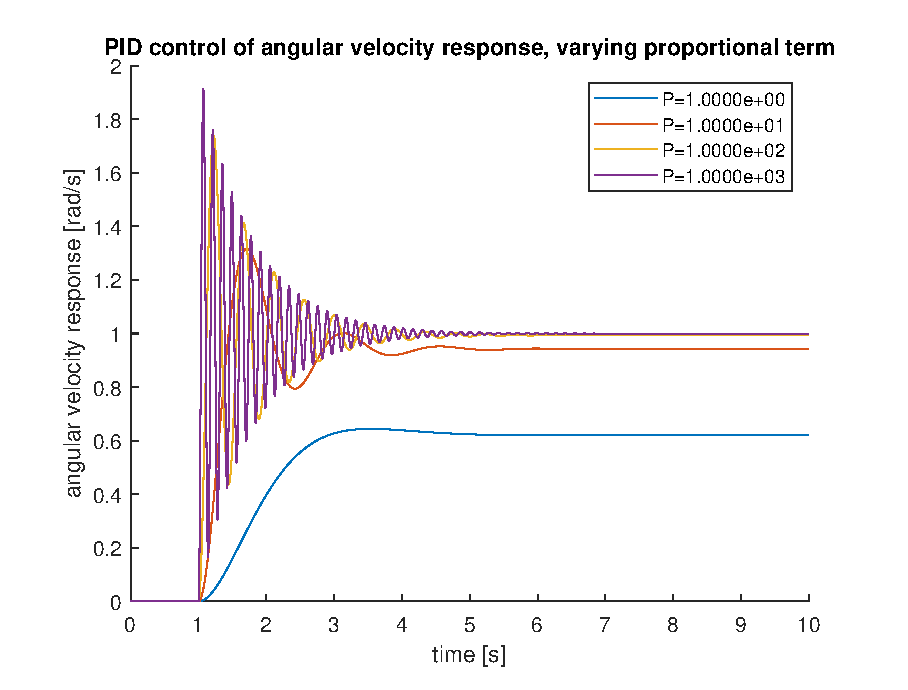
\includegraphics[width=\linewidth]{img/task01_varying_p.eps}
    \caption{Effect of the proportional term the angular velocity response in a proportional controller.}
    \label{fig:p on angular velocity}
\end{figure}

The effect of the proportional term on the response is twofold.
\begin{enumerate}
    \item There is a diminishing effect on the amplitude of the signal, but the percent overshoot continues to increase.
    \item The system becomes less damped to the point of increasing in oscillations as the $P$ term increases.
\end{enumerate}

\subsection{Task 2 -- Varying the proportional, integral terms}

\begin{figure}
    \centering
    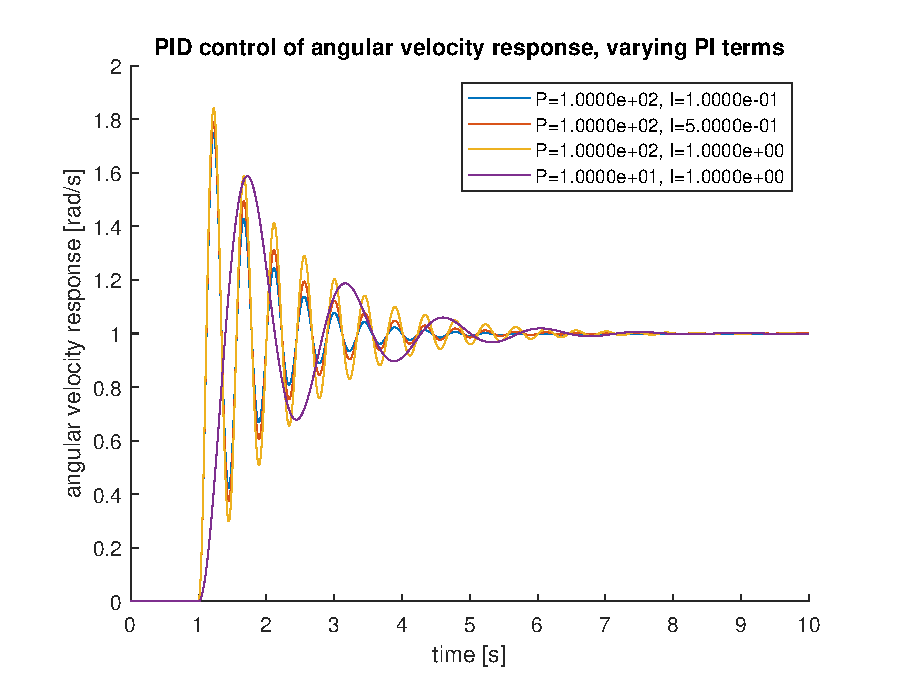
\includegraphics[width=\linewidth]{img/task02_varying_pi.eps}
    \caption{Effect of the proportional and integral terms the angular velocity response in a PI controller.}
    \label{fig:pi on angular velocity}
\end{figure}

The integral term has no effect on damping, it only changes the percent overshoot, but the number of oscillations remains the same. The change that we see in the last curve is because of the decrease in the proportional term.

\subsection{Task 3 -- Varying the proportional terms}

\begin{figure}
    \centering
    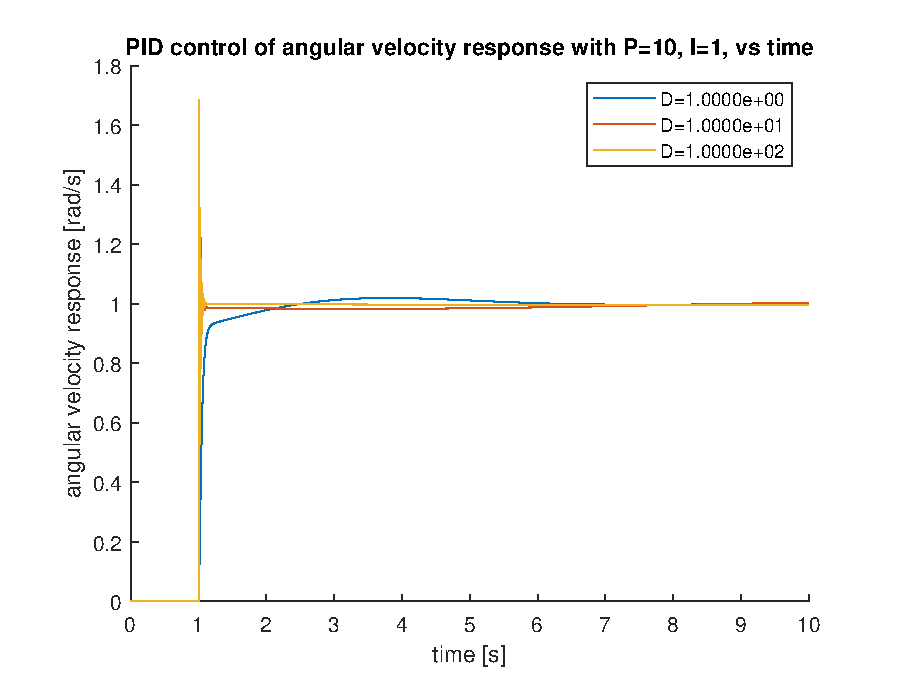
\includegraphics[width=\linewidth]{img/task03_varying_d.eps}
    \caption{Effect of the derivative term the angular velocity response in a PID controller.}
    \label{fig:d on angular velocity}
\end{figure}

All of these curves seem to have very quick settling times. The difference is that the derivative term creates a very dramatic effect on the percent overshoot. However, unlike the derivative term, it settles much more quickly.

\section{Discussion}

The difference between an ideal and a proportional PID controller is that a parallel uses the compensator

We can see the general form of the compensator formula here, that is
\begin{equation}
    P + I\frac1s + D\frac{N}{\displaystyle1 + N\frac1s}
\end{equation}
rather than
\begin{equation}
    P\brao*{1 + I\frac1s + D\frac{N}{\displaystyle1 + N\frac1s}}.
\end{equation}

The effect of this is that the proportional term only affects the proportional transfer function, rather than creating a gain on the integral and derivative term as well.

The PID controller creates very different results, and which parameters you decide on depends on the application that you desire to create.

For example, a cruise control, I would say that the best control would be a control with $P < 10$, $I < 1$, and $D = 0$. This would create very steady curves with very little overshoot or change in magnitude which would be ideal for cruise control.

On the other hand, a system that needs quick responses may want to use a much higher derivative term such as $D=100$. Depending on whether the system should take a longer time to return to equilibrium, in the case that this is required, then the system should also increase its integral term.

It would have been interesting to program the PID Controller in Verilog,
but I do not know about Verilog's capabilities with floating-point representations of real numbers.
This would make for an interesting alternative solution though.

Also, I began attempting to do a Bode plot for tasks 01--03,
but I could not finish that task
as Matlab does not have a built-in numerical Laplace transform function
and building one myself would be well outside of the scope of this experiment.

\newpage
\printbibliography

\newpage
\appendix
\section{Appendix}\label{app}

\subsection{Task 00 -- Initial parameters, Matlab script}\label{sap:initial params}
\inputminted{matlab}{src/lab09_task00_initial_dc_motor_motor_params.m}

\hr{}

\subsection{Task 01 -- Varying proportional terms, Matlab script}\label{sap:vary p}
\inputminted{matlab}{src/lab09_task01_vary_p.m}

\hr{}

\subsection{Task 02 -- Varying proportional, integral terms, Matlab script}\label{sap:vary pi}
\inputminted{matlab}{src/lab09_task02_vary_i.m}

\hr{}

\subsection{Task 03 -- Varying derivative terms, Matlab script}\label{sap:vary d}
\inputminted{matlab}{src/lab09_task03_vary_d.m}

\end{document}
